\section{Front End: Glowing Bear}
\label{sec:interoplayer-gb}

% overview
The front end we chose to use, Glowing Bear, is modified to support the PIC-SURE API in addition to the existing support of the tranSMART REST API v2.
This section describes the execution flow of Glowing Bear with PIC-SURE only, as the support for tranSMART is preexisting.
For each part, we first describe the workflow in its final form, and then which implementation steps are taken to reach that stage.

\subsection{Initialization}

% configuration
The very first step is reading the configuration, which defines the mode in which the running instance is running: tranSMART or PIC-SURE; and the corresponding authentication process to use.
It also allows to enable or disable certain features, according to the back end compatibility.
The features that can be controlled this way are:
\begin{enumerate*}
    \item query saving,
    \item data table,
    \item query subscription,
    \item data analysis,
    \item data export,
    \item observation count,
    \item variable selection,
\end{enumerate*}
which are all disabled when using PIC-SURE.

% login / pic-sure resource
After the configuration is loaded, Glowing Bear checks the validity of the token and redirects the user to the Keycloak login page if invalid or not present.
After the login is successful Glowing Bear gets the list of available data sources with the PIC-SURE API and extracts the definition of the data source it is configured to use (see~\ref{sec:bg-picsure}).


\subsubsection{Implementation}

% configuration
The following configuration options are added:
\begin{itemize}
    \setlength\itemsep{0em}

    % mode
    \item \verb|endpoint-mode|: use tranSMART or PIC-SURE mode
    \item \verb|picsure-data-source-name|: PIC-SURE data source to use
    \item \verb|force-i2b2-nesting-style|: force the i2b2 AND/OR query format
    \item \verb|enable-greedy-tree-loading|: controls whether the tree of query terms should be loaded entirely during initialization \\

    % oidc
    \item \verb|authentication-service-type|: controls the type of authentication service used
    \item \verb|oidc-server-url|: URL of the OpenID Connect server
    \item \verb|oidc-client-id|: client identifier to use with the OIDC server \\
    
    % enable disable features
    \item \verb|show-observation-counts|: controls the display of the observation counts
    \item \verb|include-query-saving|: controls the use of the query saving feature
    \item \verb|include-data-table|: controls the use of the data table feature
    \item \verb|include-query-subscription|: controls the use of the query subscription feature
    \item \verb|include-variable-selection|: controls the use of the variable selection feature
    \item \verb|enable-analysis|: controls the display of the analysis tab
    \item \verb|enable-export|: controls the display of the export tab

\end{itemize}

% PIC-SURE resource implementation overview and resource fetching
We make the code agnostic to the differences between tranSMART and PIC-SURE except from a single service, the \emph{Resource Service}, which acts as an interface between the core Glowing Bear code and the API-specific code.
The use of one or another service is controlled by a configuration option.
We factor away into the \emph{API Endpoint Service} the methods that handle the HTTP calls from the \emph{tranSMART Resource Service}, so that they can be used in the newly implemented \emph{PIC-SURE Resource Service}.
At initialization this service fetches the definition of the PIC-SURE data sources available, and implements the PIC-SURE API calls.


\subsection{Query Terms Tree}
\label{sec:design-tree}

% initialization & browsing
Right after Glowing Bear is fully initialized the tree of query terms is loaded.
As PIC-SURE supports only node-per-node loading, just the root nodes are loaded. 
This behavior is controlled by a configuration option.
For this reason, the free-text search in the tree can not be used and the auto-completion feature in the query construction component is degraded and only has the pre-loaded nodes.
Then, as the user expands the nodes in the tree, calls are made to the back end to dynamically load the children nodes.

% tree structure
Each node in the tree is characterized by a unique path, which for PIC-SURE on i2b2 has the following format:
\begin{verbatim}
    /<data source name>/<i2b2 project name>/<category>/.../<concept>/
\end{verbatim}
When displaying the tree, we omit the first element of the tree (\emph{PIC-SURE data source name}) as it is constant during the runtime, specified by the configuration.

% node content
Each tree node contains the information needed to be used as a query term.
They can be of three types: \emph{concept}, \emph{modifier}, \emph{study}, or \emph{unknown}.
An unknown type node is not queryable. 
A study type node is only used by tranSMART.
A modifier type node is applied as a constraint to a concept.
The queryable nodes in i2b2 are all concepts, and are themselves subdivided in several types:
\begin{itemize}
    \setlength\itemsep{0em}
    \item \emph{Simple}: simple concept with no associated value
    \item \emph{Categorical}: concept with a categorical (i.e. enumerated) value
    \item \emph{Numerical}: concept with a numerical value
    \item \emph{Text}: concept with a free-text value
\end{itemize}
Each of those types is mapped to the appropriate user interface component, for taking the user input.
This component is displayed in the query construction component, after the tree node is drag-and-dropped from the tree.
Additionally the nodes have the information about whether they are internal nodes or tree leaves.


\subsubsection{Implementation}

% loading refactor
Originally Glowing Bear supports only a greedy loading method, that is the whole tree is loaded at initialization.
Because PIC-SURE does not support this, at least not with acceptable performance, we refactor the \emph{Tree Node Service} to load at initialization time only the root node, if specified in the configuration.
Then we add in the \emph{Tree Node Component}, which displays the tree in the UI, the ability to load dynamically the children nodes when the user expands a tree node with missing children.

% tree node type
The original tranSMART tree node implementation represents tree nodes without typing, i.e. generic objects.
To improve the code quality and enforce a common structure between the two API implementations, we create a new \emph{Tree Node Model}.
We modify the tranSMART and create the PIC-SURE API implementation so that they both produce the same \emph{Tree Node Model}.
Among the concept types originally supported, we add the types \emph{categorical option}, \emph{text}, \emph{high dimensional} and \emph{simple}.
These cover both the new i2b2 types, and a regrouping of tranSMART types for more clarity.


\subsection{Query Construction}

% intro
The user constructs her query by drag-and-dropping query terms from the tree to the query construction component.
A screenshot of Glowing Bear's UI when constructing a query is shown figure~\ref{fig:gb-screenshot}.
As the user does so, Glowing Bear might request from the back end additional information on the query terms.
Once done, and before submitting to the back end, this query is mapped to the PIC-SURE query format.

\begin{figure}[ht]
    \centering
    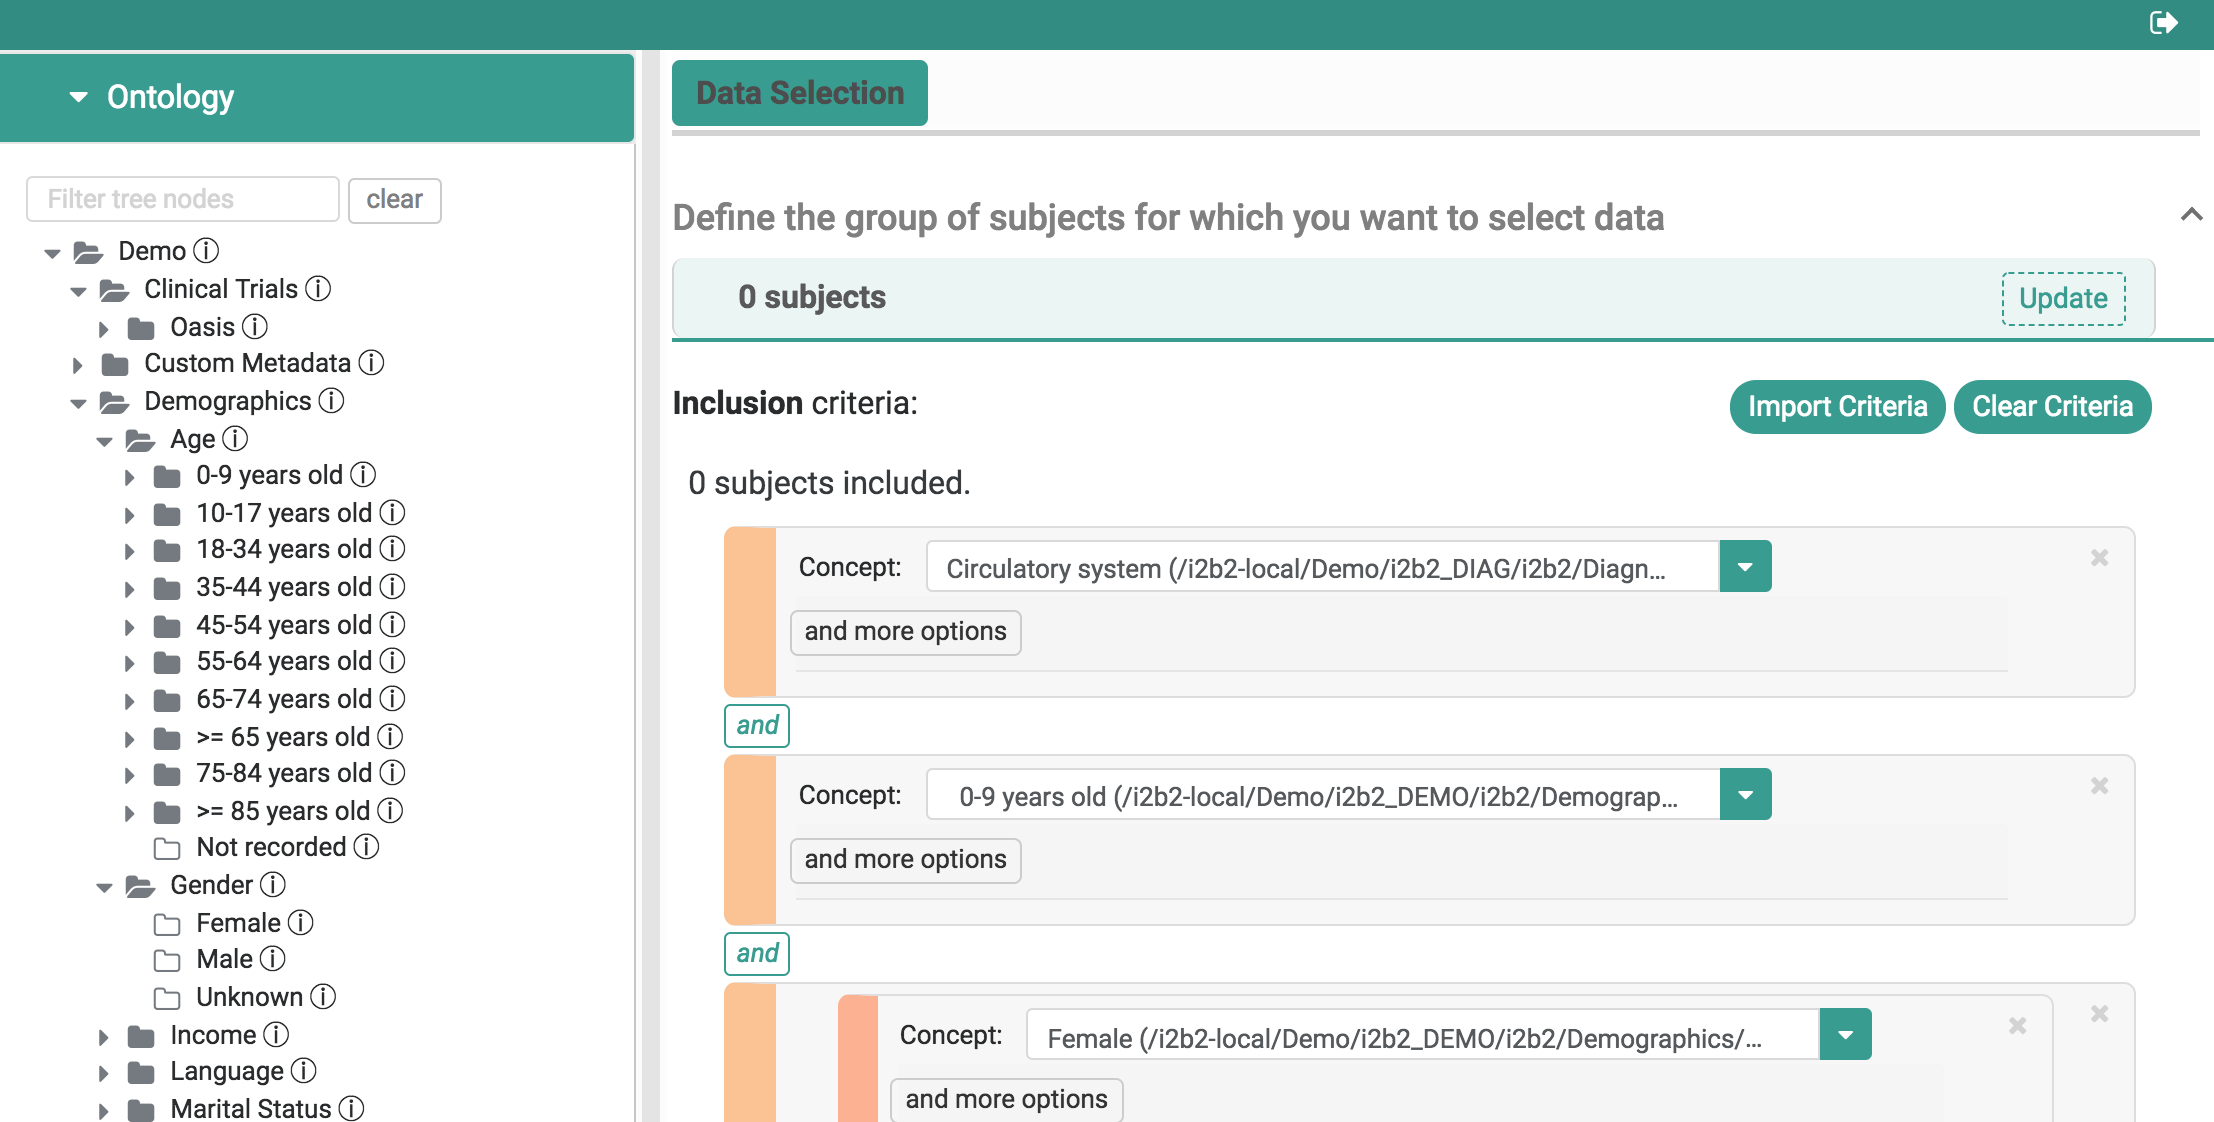
\includegraphics[width=1\textwidth]{figures/gb_screenshot.png}
    \caption{Query terms tree and query construction in Glowing Bear on i2b2}
    \label{fig:gb-screenshot}
\end{figure}

\subsubsection{Query Terms Metadata}

% intro and request
When a query term is dropped into the query construction component, a dedicated sub-component is created.
This sub-component when initialized will, according to the query term type, make a request to the back end using a tree node call with the \verb|AGGREGATE| relationship, on the term that is about to be used in the query.
With an i2b2 data source, this call is used for \emph{categorical} query terms types, as i2b2 does not have support to return aggregate values of numerical or date terms.

% answer
The answer is a usual PIC-SURE tree node answer, with additional metadata containing the categorical values.
These are then used by the sub-component to be displayed to the user.
This is an example of such an answer:

\begin{samepage}
\begin{verbatim}
{
    "pui": "/<concept path>/",
    ...
    "attributes": {
        ...
        "aggregate.categorical.0": "<categorical value 0>",
        "aggregate.categorical.1": "<categorical value 1>",
        ...
}
\end{verbatim}
\end{samepage}


\subsubsection{Generation of PIC-SURE query}
\label{sec:gb-query}

\paragraph{Data Types}
A query is a set of constraints, expressed as a list of \emph{where clauses} as explained in \ref{sec:bg-picsure}.
Since each tree node is associated to a PIC-SURE data type like explained in section~\ref{sec:design-tree}, we know through the data source definition what predicates can be applied on them.
For an i2b2 data source, here follows the data types and corresponding predicates:
\begin{itemize}
    \setlength\itemsep{0em}

    \item \emph{Simple} concept: \verb|CONTAINS|, \verb|CONSTRAIN_DATE| and \verb|MODIFIER| predicates
    \item \emph{Categorical}, \emph{Numerical} and \emph{Text} concept: the above and \verb|CONSTRAIN_VALUE|
\end{itemize}

\paragraph{Predicates}
Some predicates take values as input:
\begin{itemize}
    \setlength\itemsep{0em}

    \item \verb|CONSTRAIN_VALUE|:
    \begin{itemize}
        \item \verb|OPERATOR|: the operator to apply on the value 
        \item \verb|CONSTRAINT|: the value of the constraint
        \item \verb|UNIT_OF_MEASURE|: optionally the measure unit of the value
    \end{itemize}
    
    \item \verb|CONSTRAIN_DATE|:
    \begin{itemize}
        \item \verb|FROM_INCLUSIVE|, \verb|TO_INCLUSIVE|: if the to / from date is inclusive
        \item \verb|FROM_DATE|, \verb|TO_DATE|: date constraint boundaries
        \item \verb|FROM_TIME|, \verb|TO_TIME|: if the to / from constraint should be applied on the start or end date of the observation
    \end{itemize}
    
    \item \verb|CONSTRAIN_MODIFIER|:
    \begin{itemize}
        \item \verb|MODIFIER_KEY|: key of the modifier to be applied on the concept
    \end{itemize}
\end{itemize}

\paragraph{Example}
Assembling those together, a \emph{where clause} based on a value would be similar to the following:
\begin{samepage}
\begin{verbatim}
[{
    "field": {
        "pui": "/i2b2/project/laboratory/biochemistry/Creatinine (mg per dL)/",
        "dataType": "CONCEPT_NUMERIC"
    },
    "predicate": "CONSTRAIN_VALUE",
    "fields": {
        "OPERATOR": "GT",
        "CONSTRAINT": "4,2"
    }
}]
\end{verbatim}
\end{samepage}

\paragraph{Combination of query terms}
While tranSMART supports full freedom in the combination of query terms, i2b2 is restricted to the following format:
\begin{verbatim}
    (A OR B OR ...) AND (C OR D OR ...) AND ...
\end{verbatim}
That is, blocks of query terms linked by an \verb|AND|, where each block is internally linked by an \verb|OR|.
The restriction to this format is controlled by the configuration, and if enabled the user is forced to respect it.
In the PIC-SURE API, this translates to setting accordingly the \emph{logical operator} as such:
\begin{samepage}
\begin{verbatim}
[
    { 
        <where clause definition>,
        "logicalOperator": "AND"
    }, {
        <where clause definition>,
        "logicalOperator": "OR"
    },
    ...
]
\end{verbatim}
\end{samepage}


\subsubsection{Implementation}

% query metadata
The mechanism to request metadata about a query term from the back end is preexisting.
As such we implement the call in the \emph{PIC-SURE Resource Service} that returns the specific model that Glowing Bear expects to populate its data structures for the display and selection of the categorical variable.

% query construction
The whole process of generating queries in the PIC-SURE format are implemented in a new utility class \emph{PIC-SURE Constraint Serializer}.
Models representing the \emph{where clauses} are implemented, and the serializer is responsible to produce those, based on the Glowing Bear internal models that represent the query.

% combination
In order to restrict the format of the queries to the i2b2 format, a configuration option is added.
If enabled, the component holding the combination of query terms enforce this restriction.
The first level of nesting is always an \verb|AND|, the second level always an \verb|OR|, and no more levels are allowed.


\subsection{Query Request \& Result Retrieval}
\label{sec:interoplayer-gb-results}

% intro
After constructing the query as previously described, Glowing Bear submits the query to the back end using the \emph{PIC-SURE Query Service}.
At this stage, we are interested only in the result patient count of the query to be displayed to the user, which is what is requested in the query.

\subsubsection{Query Request}
When using only inclusion criterion, a single query is submitted as expected. 
The count returned is displayed as it is to the user.
However when using both inclusion and exclusion criterion, two query requests are actually submitted:
\begin{itemize}
    \setlength\itemsep{0em}

    \item Query 1: \verb|<inclusion criterion>|
    \item Query 2: \verb|<inclusion criterion> AND <exclusion criterion>|
\end{itemize}

Note that in the second query, the exclusion criterion is not negated.
Making two separate queries allows to display slightly more detailed counts to the user:
\begin{itemize}
    \setlength\itemsep{0em}

    \item Inclusion count: \verb|<Q1 count>|
    \item Exclusion count: \verb|<Q2 count>|
    \item Query total count: \verb|<Q1 count> - <Q2 count>|
\end{itemize}


\subsubsection{Result Retrieval}
Due to the asynchronous nature of the PIC-SURE queries, the request does not include the actual result, but the identifier of the result.
Using this identifier, Glowing Bear regularly polls the back end using the \emph{PIC-SURE Result Service} to inquire about the result status.
This status can take several values:
\begin{itemize}
    \setlength\itemsep{0em}

    \item \verb|RUNNING|: the query is still running, the regular polling continues
    \item \verb|AVAILABLE|: the query has successfully finished and the result can be requested
    \item \verb|ERROR|: the query is in error state, the polling stops and the user is informed of the error message that comes along
\end{itemize}

When the result becomes available, it is requested using the same identifier and then displayed.


\subsubsection{Implementation}

The implementation of this part is made in the Glowing Bear \emph{PIC-SURE Resource Service}, orchestrated from a single method as the core code expects synchronous count results from the query.
The result retrieval is configured to poll every second the back end for the result status, and waits up to one minute.
If after one minute the result is not available, it is considered as failed.

Additionally, because i2b2 supports only patients count and no observations count, the display of this value is disabled through the configuration.
